\documentclass[crop,tikz]{standalone}% 'crop' is the default for v1.0, before it was 'preview'
%\usetikzlibrary{...}% tikz package already loaded by 'tikz' option
\usetikzlibrary{shapes,snakes}
\usepackage{amsmath}
\begin{document}
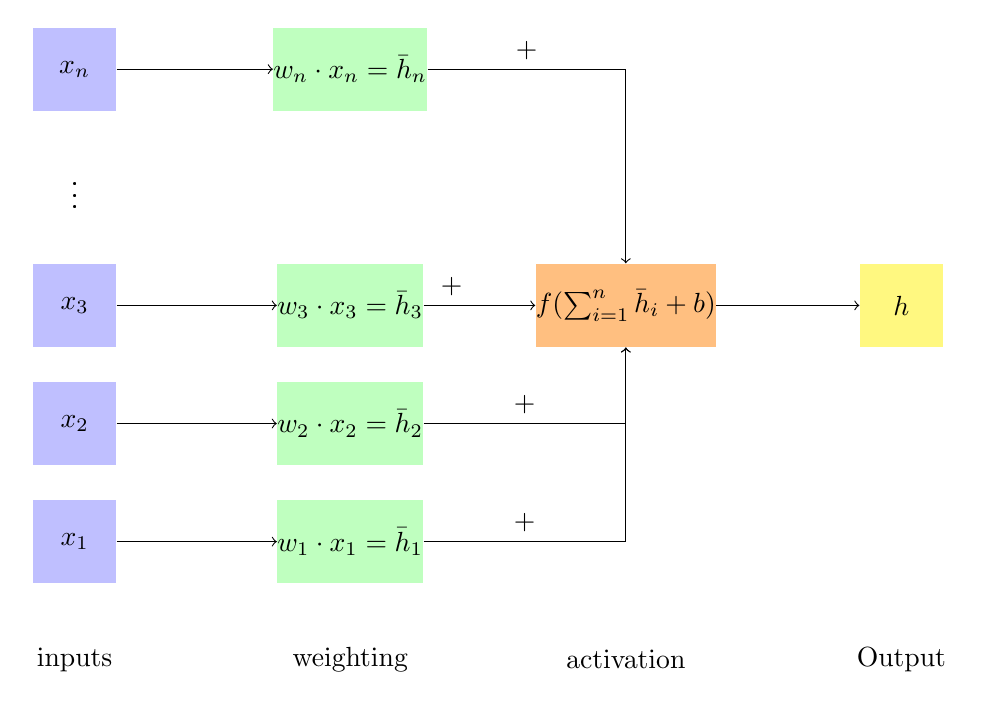
\begin{tikzpicture}

\def\vertspace{1.5cm}
\def\horispace{3.5cm}


\tikzstyle{input}=[rectangle,fill=blue!25,minimum size=30pt,inner sep=0pt]
\tikzstyle{neuron}=[rectangle,fill=green!25,minimum size=30pt,inner sep=0pt]
\tikzstyle{activation}=[neuron, fill=orange!50];
\tikzstyle{output}=[neuron, fill=yellow!50];

%inputs
\node (in) at (\horispace,-1*\vertspace) {inputs};
\node[input] (x1) at (\horispace,0*\vertspace) {$x_1$};
\node[input] (x2) at (\horispace,1*\vertspace) {$x_2$};
\node[input] (x3) at (\horispace,2*\vertspace) {$x_3$};
\node (dots) at (\horispace,3*\vertspace) {$\vdots$};
\node[input] (xn) at (\horispace,4*\vertspace) {$x_n$};

%weights
\node (nerolabel) at (2*\horispace,-1*\vertspace) {weighting};
\node[neuron] (n1) at (2*\horispace,0*\vertspace) {$w_1 \cdot x_1 = \bar{h}_1$};
\node[neuron] (n2) at (2*\horispace,1*\vertspace) {$w_2 \cdot x_2 = \bar{h}_2$};
\node[neuron] (n3) at (2*\horispace,2*\vertspace) {$w_3 \cdot x_3 = \bar{h}_3$};
\node (dots) at (\horispace,3*\vertspace) {$\vdots$};
\node[neuron] (nn) at (2*\horispace,4*\vertspace) {$w_n \cdot x_n = \bar{h}_n$};

%connections
\draw[->] (x1) -- (n1);
\draw[->] (x2) -- (n2);
\draw[->] (x3) -- (n3);
\draw[->] (xn) -- (nn);


% activation
\node (actlabel) at (3*\horispace,-1*\vertspace) {activation};
\node[activation] (act) at (3*\horispace, 2*\vertspace) {$f(\sum_{i=1}^n \bar{h}_i + b)$};

%connections
\draw[->] (n1) -| (act) node[near start, above]{+};
\draw[->] (n2) -| (act) node[near start, above]{+};
\draw[->] (n3) -- (act) node[near start, above]{+};
\draw[->] (nn) -| (act) node[near start, above]{+};

% output
\node (actlabel) at (4*\horispace,-1*\vertspace) {Output};
\node[output] (out) at (4*\horispace, 2*\vertspace) {$h$};
\draw[->] (act) -- (out);

\end{tikzpicture}
\end{document}